\documentclass[12pt,letterpaper]{memoir}
    % memoir commands to define the text block geometry
    \setulmarginsandblock{0.5in}{*}{*}
    \setlrmarginsandblock{0.5in}{*}{*} % leave space in left margin for punched holes

\usepackage{xparse}
\usepackage{blindtext}
\usepackage{xwatermark}
\usepackage{enumitem}
\usepackage{graphicx}
\usepackage{amsmath}

\usepackage{tcolorbox}
    \tcbuselibrary{skins}
\usepackage{pgfplots}
    \pgfplotsset{compat=newest}
\usepackage{tagging}

    \dashundergapssetup{
        gap-format=underline,
        teacher-gap-format=dot,
        gap-font={\ECFAugie\MTversion{augie}\color{black}},
        gap-numbers=false,
        gap-widen=true,
        gap-extend-percent=75, % note: making this too big might create errors
        gap-number-format=\,\textsuperscript{\normalfont(\thegapnumber)},
    }
    % ---------------------------------------------------------------------------
% a header to put at the top of a homework assignment
% ---------------------------------------------------------------------------
% #1 class name 
% #2 assignment number (eg, 2.5 CW)
% #3 assignment title (eg, Solve Quadratic Equations)
%
\NewDocumentCommand{\myAssignmentHeader}{ O{Algebra~2} m m }{
    \noindent
    \whenHONORS{Honors~}#1
    \hfill 
    Name : \fbox{\phantom{X\hspace{2in}}}\par
    \vspace{0.5em}
    \noindent
    {%
        \LARGE\sffamily
        \whenHONORS{H-}#2 -- #3
    }
    \hfill
    Period : \fbox{\phantom{\large 9999}}
    \hrule\hspace{\baselineskip}
    \vspace{0.5\baselineskip}
}


% ---------------------------------------------------------------------------
% I'm SO tired of writing these two explicitly!
% ---------------------------------------------------------------------------
\newcommand{\myEmph}[1]{{\bfseries\itshape#1}}

% ---------------------------------------------------------------------------
% For writing TI-84 instructions it's useful to have a visually
% distinct way to format the keys.
% ---------------------------------------------------------------------------
\newcommand{\myKey}[1]{{\ttfamily [#1]}}

\newcommand{\myDesmos}{{\scshape Desmos~}}
\newcommand{\myTi}{{\scshape TI-84~}}

% ---------------------------------------------------------------------------
% Teachers vs. Students ("tstu")
% ---------------------------------------------------------------------------
\newif\iftstu

% Typically, I will set one of these ONCE at the top of the doc.
\newcommand{\forTEACHER}{%
    \tstutrue%
    \dashundergapssetup{teacher-mode=true,}%
}
\newcommand{\forSTUDENT}{%
    \tstufalse%
    \dashundergapssetup{teacher-mode=false,}%
}

% These will conditionally generate output (the argument) based on 
% whether this document is "for" HONORS or ONLEVEL according to the previous commands.
%
% #1 the content 
% #2 text color
\NewDocumentCommand{\whenTEACHER}{ O{red} m }{\iftstu{\ECFAugie\color{#1}#2}\else{}\fi}
\newcommand{\whenSTUDENT}[1]{\iftstu{}\else{#1}\fi}



% ---------------------------------------------------------------------------
% command for creating a 1- or 2-question warmup problem
%
% #1 date
% #2 optional general directions
%
% ---------------------------------------------------------------------------
\NewDocumentEnvironment{myWarmupProblems}{ 
        O{
            \begin{itemize}
                \item Show {\itshape all} your work.
                \item Put a \fbox{box} around your answer.
            \end{itemize}
            \vspace{0.5em}
        } 
    }
{
    \newpage
    {
        \sffamily
        \begin{center}
            {
                \huge\bfseries%
                \whenHONORS{Honors~}Algebra 2 Warmup
            }%
            \\[0.5em]
            {\Large\itshape\printdate}
        \end{center}
        \noindent{\Large#1}
    }
    \large
}{
}


% ---------------------------------------------------------------------------
% A centered tcolorbox
% ---------------------------------------------------------------------------
%
% #1 - optional options to pass to tcolorbox
% #2 - the contents to put in the box
%
\NewDocumentEnvironment{myCenteredBox}{ O{} m }{%
    \begin{center}
        \begin{tcolorbox}[#1]#2\end{tcolorbox}
    \end{center}
}

% ---------------------------------------------------------------------------
% Split the output into two (roughly) equally sized side-by-side minipages.
% ---------------------------------------------------------------------------
%
% #1 - content of first minipage
% #2 - content of second minipage
%
\NewDocumentCommand{\myTwoMinipages}{mm}{
    \begin{minipage}{0.49\textwidth}
        #1
    \end{minipage}
    % \hfill 
    \begin{minipage}{0.49\textwidth}
        #2
    \end{minipage}
}


% ---------------------------------------------------------------------------
% A version of \sqrt 
% ---------------------------------------------------------------------------
%
% #1 index of the root
% #2 uproot amount
% #3 radicand
%
\NewDocumentCommand{\myRoot}{ o O{2} m  }{%
    \IfNoValueTF{#1}{\sqrt{#3\,}}{\sqrt[\uproot{#2}#1]{#3\,}}
}


% ---------------------------------------------------------------------------
% changes to part/chapter/section
% I am piggybacking Units and Lessons on Latex Parts and Chapters, respectively. 
% ---------------------------------------------------------------------------

% Here are some of the macros that capture "my settings".
\newcommand{\myPartName}{Unit}      % what I'll replace "Unit" with.
\newcommand{\myChapterName}{Lesson} % what I'll replace "Chapter" with.
\newcommand{\myLessonSuffix}{}      % a suffix after lesson (chapter) numbers (eg, 'a' in Lesson 5.2a)

% Redefine the Latex part and chapter names to use "my settings".
\renewcommand{\partname}{\myPartName}       % "Unit 2" instead of "Part II"
\renewcommand{\thepart}{\arabic{part}}
\renewcommand{\chaptername}{\myChapterName} % "Lesson 2" instead of "Chapter 2"

% A \chapter-based command to generate a lesson.
% This is a thin wrapper around \chapter that allows me
% to explicitly specify the lesson number. 
%
% #1 lesson name
% #2 optional lesson number (eg, the '2' in Lesson 5.2)
% #3 optional lesson suffix (eg, the 'a' in Lesson 5.2a)
%
\NewDocumentCommand{\myLesson}{ m O{1} O{} }
{
    \setcounter{chapter}{#2-1}
    \renewcommand{\myLessonSuffix}{#3}
    \chapter{#1}
}

% remove chapter numbers from section numbering
\makeatletter
\renewcommand\thesection{\@arabic\c@section}
\makeatother

% simulate a part without typesetting one
% 
% #1 - the part (unit) number
% #2 - the part (unit) title
\newcommand{\dummypart}[2]{%
    \setcounter{part}{#1}
    \partmark{#2}
}

% ---------------------------------------------------------------------------
% These are "annotations", the foundation of the blocked-in-text that I use.
%
% I use the term "annotations" to capture the common
% infrastructure I use to define Objectives, Vobabulary & Concepts.
% ---------------------------------------------------------------------------

% font and styling commands for
% Objectives, Voculary, Key Concepts, etc...
\newcommand{\myAnnotationStyling}{\bfseries\large}

% #1 : name of the kind of annotation (Objectives, ...)
% #2 : title text to go with the annotation
% #3 : extra tcolorbox options
%
\NewDocumentEnvironment{myAnnotate}{ m m O{}}{
    \begin{tcolorbox}[
        colbacktitle=blue!10!white,
        colback=white,
        coltitle=black,
        fonttitle={\myAnnotationStyling},
        title={#1:~},
        after title={\normalfont\itshape#2},
        #3,
        ]
}{
    \end{tcolorbox}
}

% #1 : name of the kind of annotation 
% #2 : title 
%
\NewDocumentEnvironment{myTabularAnnotate}{ m m }{
    \begin{myAnnotate}{#1}{#2}
    \begin{tabular}{r|l}
}{
    \end{tabular}
    \end{myAnnotate}
}
% #1 - column 1 text
% #2 - column 2 text
%
\NewDocumentCommand{\myRow}{mm}{{\bfseries\itshape \textcolor{blue}{#1}}&#2\\[1ex]}

% #1 : name of the kind of annotation 
% #2 : title 
% #3 : text before the list starts
%
\NewDocumentEnvironment{myListAnnotate}{ m m o }{
    \begin{myAnnotate}{#1}{#2}
    \IfValueT{#3}{#3}
    \begin{enumerate}[itemsep=0pt,fullwidth,]
}{
    \end{enumerate}
    \end{myAnnotate}
}
% #1 - column 1 text
% #2 - column 2 text
%
\NewDocumentCommand{\myItem}{mm}{\item{\bfseries\itshape \textcolor{blue}{#1}} #2}


% ---------------------------------------------------------------------------
% A table for systems of equations word problems.
%
% #1 scale factor
% ---------------------------------------------------------------------------
\NewDocumentCommand{\mySystemTable}{O{8}}{
    \begin{center}
        \begin{tabular}{|m{5em}|m{2in}|m{2in}|m{1.5in}|}
            \hline
            {\bfseries\itshape variables} & {\bfseries\itshape equations} & {\bfseries\itshape system} & {\bfseries\itshape augmented matrix} \\
            \hline\hline
            \scalebox{#1}{\fontsize{32pt}{0pt}\selectfont \phantom{\textbf{I}}} & \phantom{X} & \phantom{X} & \phantom{X}\\
            \hline
        \end{tabular}
    \end{center}
}

\NewDocumentCommand{\myBetterSystemTable}{O{4}}{
    \begin{center}
        \begin{tabular}{|m{3.25in}|m{3.25in}|}
            \hline
            \underline{\bfseries\itshape variables:} & \underline{\bfseries\itshape system of equations:}  \\
            \scalebox{#1}{\fontsize{32pt}{0pt}\selectfont \phantom{\textbf{I}}} & \phantom{X} \\
            \hline
            \underline{\bfseries\itshape augmented matrix:} & \underline{\bfseries\itshape RREF matrix:} \\
            \scalebox{#1}{\fontsize{32pt}{0pt}\selectfont \phantom{\textbf{I}}} & \phantom{X} \\
            \hline
        \end{tabular}
    \end{center}
}
    \usepackage{xparse}
\usepackage{blindtext}
\usepackage{xwatermark}
\usepackage{enumitem}
\usepackage{graphicx}
\usepackage{amsmath}

\usepackage{tcolorbox}
    \tcbuselibrary{skins}
\usepackage{pgfplots}
    \pgfplotsset{compat=newest}
\usepackage{tagging}

% ---------------------------------------------------------------------------
% x-y graphs using Tkz
% ---------------------------------------------------------------------------

% a simple "symmetric" x-y graph
%
% #1 scale of the full graph
% #2 max/min x
% #3 max/min y (optional, if absent it defaults to the x argument)
%
\NewDocumentCommand{\mySymmetricGraph}{ O{0.5} m o }{
    \begin{tikzpicture}[
        scale=#1,
        xaxe style/.style = { very thick, arrows={-{Straight Barb}}, },                 
        yaxe style/.style = { very thick, arrows={-{Straight Barb}}, },                 
        ]
        \tkzInit[
            xmax=#2, xmin=-#2, xstep=1,
            ymax=\IfValueTF{#3}{#3}{#2}, ymin=-\IfValueTF{#3}{#3}{#2}, ystep=1,
            ]
        \tkzGrid[ sub, subxstep=1, subystep=1, ]
        \tkzDrawX[label={$x$},color=black, right=0.2em,]
        \tkzDrawY[label={$y$},color=black, above=0.2em,]
        % \tkzLabelX[orig=false,]
        % \tkzLabelY[orig=false,]
        % \tkzFct[{-(},solid,very thick,color=black,samples=50,domain =-6:6.5]{\x}
    \end{tikzpicture}
}
% A counter to number the problems in the guided notes.
\newcounter{MyProblemCounter}
\setcounter{MyProblemCounter}{1}
\newcommand{\useMyProblemCounter}{\theMyProblemCounter\stepcounter{MyProblemCounter}}


\newcommand{\myProblemFont}{\bfseries\itshape}



% ---------------------------------------------------------------------------
% These are the commands I use to format the problems in the guided notes
% that have an empty space where I will write during class.
% ---------------------------------------------------------------------------

% A single problem that takes half the page.
%
% #1 : optional directions for the problem(s)
% #2 : details for problem 1
% #3 : optional font style for box titles
% #4 : vertical height of the problem boxes
% #5 : optional text at the bottom
%
\NewDocumentCommand{\myProblem}{ o m O{\large} m O{} }{%
    \IfValueT{#1}{\vspace{1\parskip}\noindent#1\nopagebreak}%
    \begin{tcbraster}[%
        raster equal height,%
        raster columns=2,%
        raster column skip=0.5mm,%
        raster row skip=0.5mm,%
        ]%
        % This is the first problem.
        \begin{tcolorbox}[%
            enhanced,%
            sharp corners,%
            colback=white,%
            coltitle=black, colbacktitle=black!10!white,%
            boxrule=0pt, borderline={0.5pt}{0pt}{black},%
            title={\texttt{\useMyProblemCounter}},%
            attach boxed title to top left%
            ]
            #3#2
            \tcblower\vspace{#4}#5
        \end{tcolorbox}
        %
        % There IS no second problem. So make it empty space.
        \begin{tcolorbox}[colback=white, colframe=white,]\end{tcolorbox}%
    \end{tcbraster}
}

% A single problem that takes the full width of the page.
%
% #1 : optional directions for the problem(s)
% #2 : details for problem 1
% #3 : optional font style for box titles
% #4 : vertical height of the problem boxes
% #5 : optional text at the bottom
%
\NewDocumentCommand{\myWideProblem}{ o m O{\large} m O{} }{%
    \IfValueT{#1}{\vspace{1\parskip}\noindent#1\nopagebreak}%
    \begin{tcbraster}[%
        raster equal height,%
        raster columns=1,%
        raster column skip=0.5mm,%
        raster row skip=0.5mm,%
        ]%
        % This is the first problem.
        \begin{tcolorbox}[%
            enhanced,%
            sharp corners,%
            colback=white,%
            coltitle=black, colbacktitle=black!10!white,%
            boxrule=0pt, borderline={0.5pt}{0pt}{black},%
            title={\texttt{\useMyProblemCounter}},%
            attach boxed title to top left%
            ]
            #3#2
            \tcblower\vspace{#4}#5
        \end{tcolorbox}
    \end{tcbraster}
}

% Two problems next to each other.
%
% #1 : optional directions for the problem(s)
% #2 : details for problem 1
% #3 : details for problem 2
% #4 : optional font style for box titles
% #5 : vertical height of the problem boxes
% #6 : optional text at the bottom of problem 1
% #7 : optional text at the bottom of problem 2
%
\NewDocumentCommand{\myProblems}{ o m m O{\large} m O{} O{#6} }{%
    \IfValueT{#1}{\vspace{1\parskip}\noindent#1\nopagebreak}%
    \begin{tcbraster}[%
        raster equal height,%
        raster columns=2,%
        raster column skip=0.5mm,%
        raster row skip=0.5mm,%
        ]%
        % This is the first problem.
        \begin{tcolorbox}[%
            enhanced,%
            sharp corners,%
            colback=white,%
            coltitle=black, colbacktitle=black!10!white,%
            boxrule=0pt, borderline={0.5pt}{0pt}{black},%
            title={\texttt{\useMyProblemCounter}},%
            attach boxed title to top left%
            ]
            #4#2
            \tcblower\vspace{#5}#6
        \end{tcolorbox}
        % This is the second problem. 
        \begin{tcolorbox}[%
            enhanced,%
            sharp corners,%
            colback=white,%
            coltitle=black, colbacktitle=black!10!white,%
            boxrule=0pt, borderline={0.5pt}{0pt}{black},%
            title={\texttt{\useMyProblemCounter}},%
            attach boxed title to top left%
            ]
            #4#3
            \tcblower\vspace{#5}#7
        \end{tcolorbox}
    \end{tcbraster}
}

% ---------------------------------------------------------------------------
% These are the commands I use to format the problems in the guided notes
% that have an partially filled space where I will also write during class.
%
% I use the term "with content" to refer to this partially filled space.
% ---------------------------------------------------------------------------

% A single problem that takes half the page.
%
% #1 : optional directions
% #2 : the problem contents
% #3 : optional font style for the content
%
\NewDocumentCommand{\myProblemWithContent}{ o m O{\large} }{%
    \IfValueT{#1}{\vspace{1\parskip}\noindent#1\nopagebreak}%
    \begin{tcbraster}[%
        raster equal height,%
        raster columns=2,%
        raster column skip=0.5mm,%
        raster row skip=0.5mm,%
        ]%
        % This is the first problem.
        \begin{tcolorbox}[%
            enhanced,%
            sharp corners,%
            colback=white,%
            coltitle=black, colbacktitle=black!10!white,%
            boxrule=0pt, borderline={0.5pt}{0pt}{black},%
            title={\texttt{\useMyProblemCounter}},%
            attach boxed title to top left%
            ]
            #3#2
        \end{tcolorbox}
        %
        % There IS no second problem. So make it empty space.
        \begin{tcolorbox}[colback=white, colframe=white,]\end{tcolorbox}%
    \end{tcbraster}
}


% Two problems that that sit next to each other.
%
% #1 : optional directions
% #2 : the 1st problem contents
% #3 : the 2nd problem contents
% #4 : optional font style for the content
%
\NewDocumentCommand{\myProblemsWithContent}{ o m m O{\large} }{%
    \IfValueT{#1}{\vspace{1\parskip}\noindent#1\nopagebreak}%
    \begin{tcbraster}[%
        raster equal height,%
        raster columns=2,%
        raster column skip=0.5mm,%
        raster row skip=0.5mm,%
        ]%
        % This is the first problem.
        \begin{tcolorbox}[%
            enhanced,%
            sharp corners,%
            colback=white,%
            coltitle=black, colbacktitle=black!10!white,%
            boxrule=0pt, borderline={0.5pt}{0pt}{black},%
            title={\texttt{\useMyProblemCounter}},%
            attach boxed title to top left%
            ]
            #4#2
        \end{tcolorbox}
        % This is the second problem.
        \begin{tcolorbox}[%
            enhanced,%
            sharp corners,%
            colback=white,%
            coltitle=black, colbacktitle=black!10!white,%
            boxrule=0pt, borderline={0.5pt}{0pt}{black},%
            title={\texttt{\useMyProblemCounter}},%
            attach boxed title to top left%
            ]
            #4#3
        \end{tcolorbox}
    \end{tcbraster}
}


% A wide problem that can have any latex code in the content area of the box.
%
% #1 : optional directions 
% #2 : the problem
% #3 : optional font style for the content
%
\NewDocumentCommand{\myWideProblemWithContent}{ o m O{\large} }{%
    \IfValueT{#1}{\vspace{1\parskip}\noindent#1\nopagebreak}%
    \begin{tcbraster}[%
        raster equal height,%
        raster columns=1,%
        raster column skip=0.5mm,%
        raster row skip=0.5mm,%
        ]  
        \begin{tcolorbox}[%
            enhanced,%
            sharp corners,%
            colback=white,%
            coltitle=black, colbacktitle=black!10!white,%
            boxrule=0pt, borderline={0.5pt}{0pt}{black},%
            title={\texttt{\useMyProblemCounter}},%
            attach boxed title to top left%
            ]%
            #3#2
        \end{tcolorbox}
    \end{tcbraster}
}

\forHONORS
\forSTUDENTorTEACHER % which one? it depends on an env. var. (defined in the build recipe)



\begin{document}
\pagestyle{empty}
\checkandfixthelayout
\raggedbottom

%-----------------------------------------------------------------------------------------
\myAssignmentHeader{9.1}{Shoe Size Regression Activity}
%-----------------------------------------------------------------------------------------

\subsection*{Creating a Scatterplot}

\begin{enumerate}[fullwidth,label={\Large$\bm{\square}$}\,\arabic*.]
    \item Write down your \myEmph{shoe size}: \underline{\hspace{1in}} 
        {\scshape Men}
        \quad 
        {\scshape Women} (circle one)
    \item Calculate your \myEmph{foot length} from your shoe size: \underline{\hspace{1in}} inches
            \includegraphics[width=0.75in]{QR-shoe-size-conversion}
            \raisebox{0.25in}{\tiny\itshape (Shoe size calculator)} 
    \item Write down your \myEmph{height}: \underline{\hspace{1in}} inches
    \item Add your {\itshape foot length} and {\itshape height} to the \myEmph{class data} on the whiteboard.
    \item Copy all the class data from the whiteboard into the \myEmph{table} below.
    \item Sketch a \myEmph{scatterplot} by plotting the points in your table on the graph on the next page.
\end{enumerate}

\begin{minipage}{0.35\textwidth}
    \centering
    \renewcommand{\arraystretch}{1.25}
    \begin{tabular}{|m{1in}|m{1in}|}
        \hline
        \myEmph{x (foot len.)} & \myEmph{y (height)} \\
        \hline
        \quad & \quad \\ \hline%
        \quad & \quad \\ \hline%
        \quad & \quad \\ \hline%
        \quad & \quad \\ \hline%
        \quad & \quad \\ \hline%
        \quad & \quad \\ \hline%
        \quad & \quad \\ \hline%
        \quad & \quad \\ \hline%
        \quad & \quad \\ \hline%
        \quad & \quad \\ \hline%
        \quad & \quad \\ \hline%
        \quad & \quad \\ \hline%
        \quad & \quad \\ \hline%
        \quad & \quad \\ \hline%
        \quad & \quad \\ \hline%
        \quad & \quad \\ \hline%
        \quad & \quad \\ \hline%
        \quad & \quad \\ \hline%
        \quad & \quad \\ \hline%
        \quad & \quad \\ \hline%
        \quad & \quad \\ \hline%
    \end{tabular}
\end{minipage}
\begin{minipage}{0.64\textwidth}
    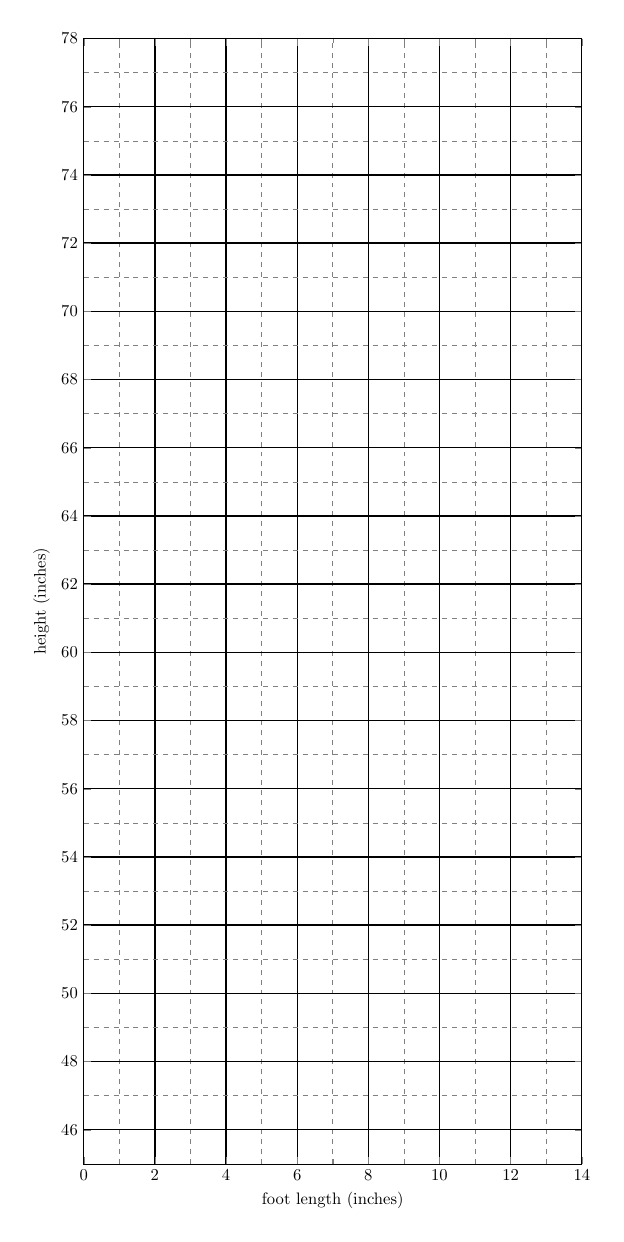
\begin{tikzpicture}[scale=0.6]
        \begin{axis}[
            xmin = 0, xmax = 14,
            ymin = 45, ymax = 78,
            % xtick distance = 2.5,
            % ytick distance = 0.5,
            grid = both,
            minor tick num = 1,
            major grid style = {thick,black},
            minor grid style = {dashed,black!50},
            width = \textwidth,
            height = 10in,
            xlabel = {foot length (inches)},
            ylabel = {height (inches)},
            legend cell align = {left},
        ]
        \end{axis}
    \end{tikzpicture}

\end{minipage}


\subsection*{Line of Best Fit}

\begin{enumerate}[fullwidth,label={\Large$\bm{\square}$}\,\arabic*.,resume]
    \item Which shape do you think ``best fits'' the dots? (circle one)
        \begin{tcbraster}[
            raster equal height, raster columns = 3,
            raster left skip = 0.3in, raster right skip = 0.3in, raster column skip = 0.2in,
            colback=white, valign=center,
        ]
            \begin{tcolorbox}
                \centering
                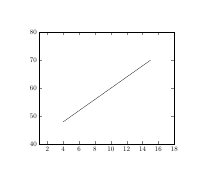
\begin{tikzpicture}[scale=0.25]
                    \begin{axis}[
                        ymin = 40, ymax = 80,
                        xmin = 1, xmax = 18]
                        \addplot[domain = 4:15,] {2*x + 40};
                    \end{axis}
                \end{tikzpicture}\\
                \myEmph{Linear}
            \end{tcolorbox}
            \begin{tcolorbox}
                \centering
                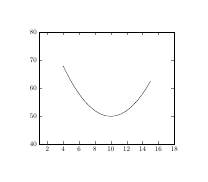
\begin{tikzpicture}[scale=0.25]
                    \begin{axis}[
                        ymin = 40, ymax = 80,
                        xmin = 1, xmax = 18]
                        \addplot[domain = 4:15,] {0.5*(x-10)^2+50.0};
                    \end{axis}
                \end{tikzpicture}\\
                \myEmph{Quadratic}
            \end{tcolorbox}
            \begin{tcolorbox}
                \centering
                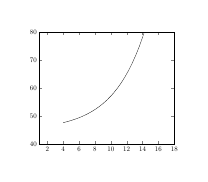
\begin{tikzpicture}[scale=0.25]
                    \begin{axis}[
                        ymin = 40, ymax = 80,
                        xmin = 1, xmax = 18]
                        \addplot[domain = 4:15,] {exp(0.25*x)+45};
                    \end{axis}
                \end{tikzpicture}\\
                \myEmph{Exponential}
            \end{tcolorbox}
        \end{tcbraster}
    \item Use a ruler to draw a \myEmph{line of best fit} that you think almost goes through all the points.
    \item Estimate the \myEmph{slope} and \myEmph{$\bm{y}$-intercept} for your line.
        \begin{itemize}
            \item slope:
                \begin{itemize}
                    \item two points on your line: 
                        $(x_1,y_1) = $ (\underline{\hspace{4em}},\underline{\hspace{4em}})
                        $(x_2,y_2) = $ (\underline{\hspace{4em}},\underline{\hspace{4em}})
                    \item {\itshape my estimated} 
                        $m = \frac{\Delta y}{\Delta x} = \frac{y_2 - y_1}{x_2 - x_1} =$ 
                        \underline{\hspace{3in}}
                \end{itemize}
            \item $y$-intercept:
                \begin{itemize}
                    \item Where does your line cross the $y$-axis?
                    \item {\itshape my estimated} $b =$ \underline{\hspace{1in}}
                \end{itemize}
        \end{itemize}
\end{enumerate}

\subsection*{Linear Regression Analysis}

\begin{enumerate}[fullwidth,label={\Large$\bm{\square}$}\,\arabic*.,resume]
    \item Open the {\scshape Desmos} graphing calculator on your phone, or share with someone else.
    \item Create an empty {\scshape Desmos} $(x_1,y_1)$ \myEmph{table} by clicking on \fbox{\Large +}.
    \item Enter at least \myEmph{10 rows} from your table on the next page into the {\scshape Desmos} table.
        \begin{itemize}[nosep]
            \item Put {\itshape foot length} data into the $x_1$ column.
            \item Put {\itshape height} data into the $y_1$ column.
            \item How many rows did you copy? \underline{\hspace{1in}}
            \item How many dots do you see in the {\scshape Desmos} scatterplot? \underline{\hspace{1in}}
        \end{itemize}
    \item Tell {\scshape Desmos} to do a \myEmph{linear regression} 
        to find the ``best fit'' line for the scatterplot.
        Do this by entering the following formula into {\scshape Desmos}.
        \begin{itemize}[nosep]
            \item {\ttfamily y1 \raisebox{0.25em}{\large\texttildelow}\, m x1  +  b}
        \end{itemize}
    \item Write down the values of $m$ and $b$ that {\scshape Desmos} calculated.
        \begin{itemize}[nosep]
            \item {\scshape Desmos} $m =$ \underline{\hspace{0.5in}}
            \item {\scshape Desmos} $b =$ \underline{\hspace{0.5in}}
        \end{itemize}
\item Compare the values of $m$ and $b$ that {\scshape Desmos} calculated 
        to your values in step 9, above. What do you notice?
        \begin{itemize}
            \item How my slope estimate compared to {\scshape Desmos}: \hrulefill
            \item[] \hrulefill
            \item[] \hrulefill
            \item How my $y$-intercept estimate compared to {\scshape Desmos}: \hrulefill
            \item[] \hrulefill
            \item[] \hrulefill
        \end{itemize}
\end{enumerate}



\end{document}